\documentclass[showpacs,amsmath,amssymb,aps,prc,floatfix,showkeys,nofootinbib]{revtex4-1}
\pdfoutput=1 %oversteps the use of dvi or postscript

\usepackage{graphicx}% Include figure files
\usepackage{dcolumn}% Align table columns on decimal point
\usepackage{bm}% bold math
\usepackage[mathlines]{lineno}% Enable numbering of text and display math
\usepackage{mathtools}
%\linenumbers\relax % Commence numbering lines
\usepackage{relsize}
\usepackage{tikz}
\usetikzlibrary{shapes.geometric, arrows}
\usepackage{enumitem}
\usepackage{lipsum}
\usepackage{multirow}
\newcommand{\myarrow}{\tikz\draw[thick,black,-latex] (0,1) -- ++(0,-2ex) -- +(3.5ex,0);}


\usepackage{slashed}
\usepackage{hyperref}
\usepackage{url}
\usepackage{color}
\usepackage{subcaption}


\begin{document}

\section{\label{intro}Intro}
The effective use of a kinematic fitter for any nuclear/particle physics reaction requires an accurate estimate of the uncertainties of the measured kinematics (P, $\theta$, $\phi$, etc.). Unfortunately for the current state of CLAS12 tracking, we do not have valid covariance matrices. Therefore, if one wants to implement a kinematic fitter tool on CLAS12 data, it is necessary to first model the covariances across all kinematics available within the acceptance of the CLAS12 detector. To do this, we have chosen to empirically measure the covariances using full GEMC simulations. Due to kinematic dependencies of the covariances, it was decided that a binned and interpolated approach would be most appropriate. To begin this process of modeling the covariances of the CLAS12 detector, we started with the drift chambers. This decision was based on the importance of the drift chambers for most physics reactions. But a fully functioning kinematic fitter will need covariance matrices for other detectors as well (Forward Tagger, ECAL, CVT, etc.). 

\section{\label{dc_covMat}Drift Chamber Covariance Matrix Extraction}
The concept is straightforward. First, generate a single particle in the detector over the desired space. Since we are initially just measuring the DC covariances, the particles were generated over just the range covered by the forward detector. Then, reconstruct the generated single-particle events with the standard CLAS12 reconstruction software. Next, bin the data in P, $\theta$, and $\phi$. Other kinematic variables can be used, but these are the ones chosen for this project. (These are also the kinematics used in the kinematic fitter.) Finally, by comparing the reconstructed and generated values for the chosen kinematics, the DC covariance matrices for a given particle can be calculated. 

\subsection{\label{gen}Generating the Single Particle Events}
Due to the identical geometries of the magnetic fields from sector to sector, there shouldn't be any sector dependencies of the covariances for simulation. Thus, we decided to model the covariance matrices for a single sector and apply that model to all six sectors. This reduces the amount of generated events needed by a factor of six. Sector 2 was chosen to model the covariance matrix, which would then be used for all sectors. GEMC was used to generate events with a single particle per event. These were ``particle gun" simulations, i.e. the beam conditions in the gcard were modified to represent the desired particle type, energy, and vertex angle. 

All of the necessary tools to extract the covariance matrices should be located in the /covMatrix\_extraction/ directory. This includes the scripts used to generate the single particle events and the gcards. To begin, we start with the default CLAS12 gcard for GEMC 5.4: github.com/JeffersonLab/clas12-config/blob/main/gemc/5.4/clas12-default.gcard. The first two particles for which the DC covariance matrices were modeled were $\pi^+$ and $\pi^-$. An example of the modified beam conditions in the gcard is shown in Fig. \ref{fig:gcard_beam}. The gcards used in the simulations of single $\pi^+$ events and single $\pi^-$ events are located in /covMatrix\_extraction/gcards/. There are bash submission scripts in the /covMatrix\_extraction/ directory that were set up for submitting the simulation jobs via SIWF2. Currently, the steps of generating the events with GEMC and running the CLAS12 reconstruction on those events are done in separate job submissions \footnote{These can be combined into one workflow for a more streamlined process, but for now, it's in two steps.}. To generate the events with GEMC, the script is called swif2\_gemc\_jobs.sh. This script will create the output directories if they do not already exist. The output HIPO files from this workflow will be saved to \$output\_dir/gemc/. These HIPO files will be the input for for the next step of the simulation, which is the reconstruction. To do this, the swif2\_recon\_jobs.sh script can be run. Executing swif2\_recon\_jobs.sh will produce output .rec.hipo files in \$output\_dir/cooked/. The user should modify the input and output directories in the two bash scripts for their use. NOTE: Make sure that the ``output\_dir" variable is defined the same in both bash scripts.

To ensure sufficient coverage over all acceptance of sector 2, 100 million events were generated for each particle. In order to be certain that a reconstructed particle is indeed the one that we generated, truth matching is used. For truth matching information to be accessible when analyzing the reconstructed events, the following options need to be enabled in the gcard: \\
-SAVE\_ALL\_MOTHERS=1 \\
-SKIPREJECTEDHITS=1 \\
-INTEGRATEDRAW=``*"  \\
These can also be given as options when running GEMC.

Before generating the entire dataset that will be used in extracting the covariance matrices, it is a good idea to generate a smaller sample and investigate the $P$ and $\theta$ distributions. Depending on the particle type and magnetic field configuration, the acceptance coverage can vary. The optimal ranges for $P$ and $\theta$ simulations can be determined by examining these distributions. (The $\phi$ range, over which the single particle events are generated, can be the exact geometry of the sector: 30$^\circ$ to 90$^\circ$ for sector 2.) The file, kinematics\_plots.C, was set up for this exact purpose. When run, kinematics\_plots.exe will produce a ROOT file with a TTree, called kinInfoTree, that contains branches for the Rec and MC kinematic information. These distributions can be plotted to easily determine what the generated ranges should be for $P$ and $\theta$. NOTE: There are input and output directories hardcoded in the kinematics\_plots.C. The user should modify these accordingly.

\begin{figure} 
\centering
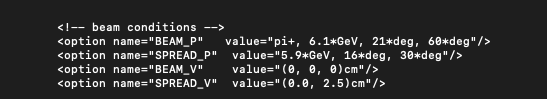
\includegraphics[width=.95\linewidth]{gcard_beam_modifications}
\caption{This screenshot shows and example of the beam specifications in the gcard. Here, a $\pi^+$ particle gun is defined. Each generated event will contain only a $\pi^+$ with an energy between 0.2 and 12 GeV, a $\theta$ between 5$^\circ$ and 37$^\circ$, and a $\phi$ between 30$^\circ$ and 90$^\circ$.}
\label{fig:gcard_beam}
\end{figure}


\subsection{\label{binning}Binning in P, $\theta$, and $\phi$} 
The more bins utilized, the better representation we'll have of the true covariances across the kinematics. But of course, more bins also means more simulations are necessary to sufficiently populate all of the bins. For now, it was decided to have 25 bins in each of the three currently used kinematics. This comes out to a total of 25$\times$25$\times$25=15,625 bins. There may be room for optimization of this binning (and possibly varying binning across kinematics), but this is currently what is done. The binning scheme is shown in Table \ref{tab:binning}. 

\begin{table}[h!]
\centering
\caption{\label{tab:binning}The binning information implemented for modeling the DC covariance matrices for $\pi^+$ and $\pi^-$ with an inbending torus field (negative particles bend toward the beamline). The maximum $\theta$ (and potentially the minimum $\theta$ for other particles) is different for $\pi^+$ and $\pi^-$. For $\pi^+$ the maximum is 37$^\circ$, and for $\pi^-$ the maximum is 40$^\circ$. These values were determined from the distribution saved with kinematics\_plots.C}
\begin{tabular}{|c|c|c|c|}
\hline
Kinematic Variable & N bins & Min & Max \\
\hline
$P$ & 25 & 0.2 [GeV] & 12 [GeV] \\
$\theta$ & 25 & 5$^\circ$ & 37$^\circ$($\pi^+$), 40$^\circ$($\pi^-$) \\
$\phi$ & 25 & 30$^\circ$ & 90$^\circ$ \\
\hline
\end{tabular}
\end{table}

\subsection{\label{covMat}Extracting Covariance from Simulations}
Once all of the single particle events are generated and reconstructed, we can analyze the results to determine the covariance matrices for the particles. The process of reading the HIPO files, calculating the covariance matrices, and saving these results bin-by-bin, is all done with a single executable file, covMatrix\_single\_particle.exe. This executable is compiled from a C++ source file, covMatrix\_single\_particle.C. Hardcoded in this file is the location of the input data directory, which should be the directory in which the HIPO files of the single-particle generated and reconstructed events are located. Also hardcoded in this file are the binning specifications. These are defined by the number of bins for each kinematic variable and the corresponding bin ranges. From these values, the bin size for each kinematic is determined. Currently, all bins for a given kinematic variable have the same size.

There is a method contained in covMatrix\_single\_particle.C, called calculateCovariance, which, as the name suggests, is where the covariance values are calculated. This is done according to eq. \ref{eq:covariance}. In this equation, $x$ and $y$ represent the kinematic variable(s) in which we are interested. For example, if we are calculating the covariance between $P$ and $\theta$, $x$ would represent $P$ and $y$ would represent $\theta$ (or vice versa). If we are calculating the variance of $\phi$, both $x$ and $y$ would represent $\phi$. The summation in eq. \ref{eq:covariance} is done event-by-event. The $\delta x_i$ term is $(Rec-MC)$, or the reconstructed value minus the generated value, for the given kinematic for a specific event. Similarly, $\delta y_i$ can be the $(Rec-MC)$ value for another kinematic variable, or the same variable if it is the variance of that variable that's being calculated. The $\mu$ terms represent the means of the $(Rec-MC)$ distributions  for the corresponding kinematic variable(s).

This calculation can be quite sensitive to outliers in the distributions. In particular, these outliers may present themselves as asymmetric, non-gaussian contributions to the distributions. The effect of this can be not only a broadening of the standard deviation (which means an overestimation of the covariance), but also a shift of the mean from the true value, which would further corrupt the covariance calculation. The outliers in these $(Rec-MC)$ distributions appear to be due to poorly reconstructed tracks. These unwanted events should not be included in the covariance calculations, and thus, a robust method for removing these outliers is necessary. To handle this, several steps are taken. But first, each of the three $(Rec-MC)$ distributions ($\delta P$, $\delta \theta$, and $\delta \phi$) are added to 1-dimensional histograms (this is done individually for each kinematic bin). Next, the histograms are rebinned according to the number of bins over the gaussian peak region using TH1::Rebin(). Since this function can only reduce the number of bins, we need to start out with enough bins so that we wont have a situation in which the number of bins should be increased. 

There are two sequential steps taken to remove the outliers. First, the interquartile range (IQR) of each $\delta$ distribution is determined with TH1::GetQuantiles(). This is the range over which the inner 50\% of the data is located. This range is less impacted by outliers than standard deviation or RMS. This range is tighter than what we ultimately want, but it serves as a good starting point from which to spread outward. To do this, a method in the covMatrix\_single\_particle.C file, called iqr\_zoom, resets the range of the histograms according to some multiplicative factor of the IQR. The factor is currently set to 5, but this can be modified in the code; the larger the number, the wider the range will be.

With the histograms zoomed in according to the IQR, the means and RMS's are extracted. These parameters will determine the final ranges for the $\delta$ distributions, over which the covariances will be calculated. This is the second step of outlier exclusion. There is an ``if" statement in the calculateCovariance method, in which it is checked that the $(Rec-MC)$ values for all of the kinematics fall within the range specific by $\mu\pm3\sigma$. Any values that fall outside of this range will not be included in the calculations of the covariances.  The means are also used directly in the calculations of the covariances (see Eqn. \ref{eq:covariance}).

The calculated covariances are stored in TH3's, which are saved to an output ROOT file. The output ROOT file is called ``C\_file" in the covMatrix\_single\_particle.C file; it's output location and name should be modified by the user in the code to whatever is desired. The 3 dimensions of the TH3's represent the bin centers for each of the 3 kinematic variables: $P$, $\theta$, and $\phi$. The value for a given 3D bin is set to the covariance value for that kinematic bin, and there is a TH3 for each of the covariance elements: $C_P$, $C_\theta$, $C_\phi$, $C_{P\theta}$, $C_{P\phi}$, $C_{\theta\phi}$. So, each of these TH3's has 15,625 entries, one for each kinematic bin. The ROOT file, in which these TH3's are stored, is read directly by the kinematic fitter.

In addition to the TH3's containing the covariance information, there is also a TH3 saved to the output ROOT file for each of the following: N entries, $\mathlarger{\mathlarger{\sigma}}_{C_{P}}$, $\mathlarger{\mathlarger{\sigma}}_{C_{\theta}}$, $\mathlarger{\mathlarger{\sigma}}_{C_{\phi}}$, $\mathlarger{\mathlarger{\sigma}}_{C_{P\theta}}$, $\mathlarger{\mathlarger{\sigma}}_{C_{P\phi}}$, $\mathlarger{\mathlarger{\sigma}}_{C_{\theta\phi}}$, $P$ offset, $\theta$ offset, and $\phi$ offset. Each of the $\mathlarger{\mathlarger{\sigma}}$ terms represent the error in the corresponding covariance matrix element. The ``offset" terms are the means of the corresponding kinematic $(Rec-MC)$ distributions; these are the same means used in the covariance calculations. Any non-zero value for the means of these distributions indicates a systematic shift for the kinematic that may need to be corrected for.

\begin{equation} \label{eq:covariance}
C_{xy}=\frac{\smashoperator[r]\sum_{i}^{N}[(\delta x_i-\mu_{\delta x})(\delta y_i-\mu_{\delta y})]}{N}
\end{equation}

The errors of the covariances are calculated following eqn. \ref{eq:cov_err} \cite{cov_err_stack_exchange}. Although these are not used in any calculations, they provide a good metric for validating some aspects of the covariance matrix elements. For example, if the covariance matrix elements have very large errors relative to their fluctuations, it may indicate that there are insufficient statistics in a given kinematic bin.

\begin{equation} \label{eq:cov_err}
\mathlarger{\mathlarger{\sigma}}_{C_{xy}}=\frac{C^2_{xy}+C_{xx}C_{yy}}{N-1}
\end{equation}

The covMatrix\_single\_particle.exe executable can be run interactively, but this should only be done when reading a small number of HIPO files, such as when testing. For reading \emph{all} of the HIPO files needed for extracting covariance matrices, this should be submitted as a job to the batch farm. There is a very simple bash script in /covMatrix\_extraction/, called covMat\_subScript, that was written to submit the covMatrix\_single\_particle.exe executable with SLURM. The resource specifications in the script were chosen based on 100M generated events, but of course these can be adjusted as needed. 

In addition to the output ROOT file containing the covariances and additional information described above, there is another ROOT file that is output which contains the information from which the covariances are calculated. This ROOT file contains a bunch of TH1's and TH2's, for all of the $(Rec-MC)$ distributions. There are six folders under the ``Histograms" directory in the ROOT file: ``delta p Histograms", ``delta theta Histograms", ``delta phi Histograms", ``delta p delta theta Histograms", ``delta p delta phi Histograms", and ``delta theta delta phi Histograms". Each folder contains 15,625 histograms, one for each kinematic bin. These allow the user to visually examine the $\delta$ distributions that are used for calculating the covariances. This is a useful tool for validating outlier exclusion, proper binning, and other distribution properties.

It is also useful to view the calculated covariances as a function of the kinematics. A file named ``covMatrix\_plots\_save\_all.C" was written to produce a PDF file containing 625 pages of scatterplots. Each page has the following six scatterplot subplots: $C_P$ vs $x$, $C_\theta$ vs $x$, $C_\phi$ vs $x$, $C_{P\phi}$ vs $x$, $C_{P\theta}$ vs $x$, and $C_{\theta\phi}$ vs $x$. The $x$ in each of these can be any one of the three kinematic variables: $P$, $\theta$, or $\phi$. The way the code is currently written, the user must specify which kinematic variable they want to view the covariances as a function of; only one can be done at a time. When covMatrix\_plots\_save\_all.exe is run, all of the scatterplots for the specified kinematic variable will be saved to a PDF, called C\_vs\_$<$kin$>$\_plots.pdf. The variable in the the covMatrix\_plots\_save\_all.C file that controls the kinematic variable that will be plotted is a std::string called ``varying\_kin". The options for varying\_kin are: ``p", ``theta", or ``phi".

\section{\label{kinFitter}CLAS12 Kinematic Fitter}





\section{References}
\begin{thebibliography}{21}
\expandafter\ifx\csname natexlab\endcsname\relax\def\natexlab#1{#1}\fi
\expandafter\ifx\csname bibnamefont\endcsname\relax
  \def\bibnamefont#1{#1}\fi
\expandafter\ifx\csname bibfnamefont\endcsname\relax
  \def\bibfnamefont#1{#1}\fi
\expandafter\ifx\csname citenamefont\endcsname\relax
  \def\citenamefont#1{#1}\fi
\expandafter\ifx\csname url\endcsname\relax
  \def\url#1{\texttt{#1}}\fi
\expandafter\ifx\csname urlprefix\endcsname\relax\def\urlprefix{URL }\fi
\providecommand{\bibinfo}[2]{#2}
\providecommand{\eprint}[2][]{\url{#2}}


\bibitem{cov_err_stack_exchange}
  \bibinfo{journal}{https://stats.stackexchange.com/questions/48366/standard-errors-for-covariance-estimate-in-r} 

  
  \end{thebibliography}


\end{document}

